\chapter{Results, Inferences, and Discussion}
\label{chap:results}

\section{Baseline Model Performance}
\label{sec:baseline_performance}

The Stacked Ensemble achieved the best overall performance, as shown in Table~\ref{tab:baseline} (Section~\ref{sec:baseline_modeling}). The test $R^2$ of 0.6433 means the model explains 64\% of the variance in \citet{Frey_Osborne_2017}'s automation scores from 100 O*NET features. While not a perfect replication (\citet{Frey_Osborne_2017} used a 2010 internal O*NET version that is no longer publicly available), this level of explanatory power demonstrates that the structural relationship between occupational characteristics and historical automation risk is highly learnable from current data.

The feature importance hierarchy reveals the model's learned structure. Fluency of Ideas (0.2177) and Originality (0.1919) dominate, confirming that \citet{Frey_Osborne_2017}'s creative intelligence bottleneck is the single strongest structural predictor of automation resistance in the 2013 data. Job Zone (0.0569), representing required education level, ranks third; higher education correlated with lower automation risk in 2013. The remaining top features include Instructing (0.0478), Active Learning (0.0372), and Deductive Reasoning (0.0326), all cognitive and social skills that the 2013 model learned to associate with automation protection. This will become ironic in the MAEI results, where precisely these cognitive skills become risk factors under 2026 conditions.

\begin{figure}[htbp]
\centering
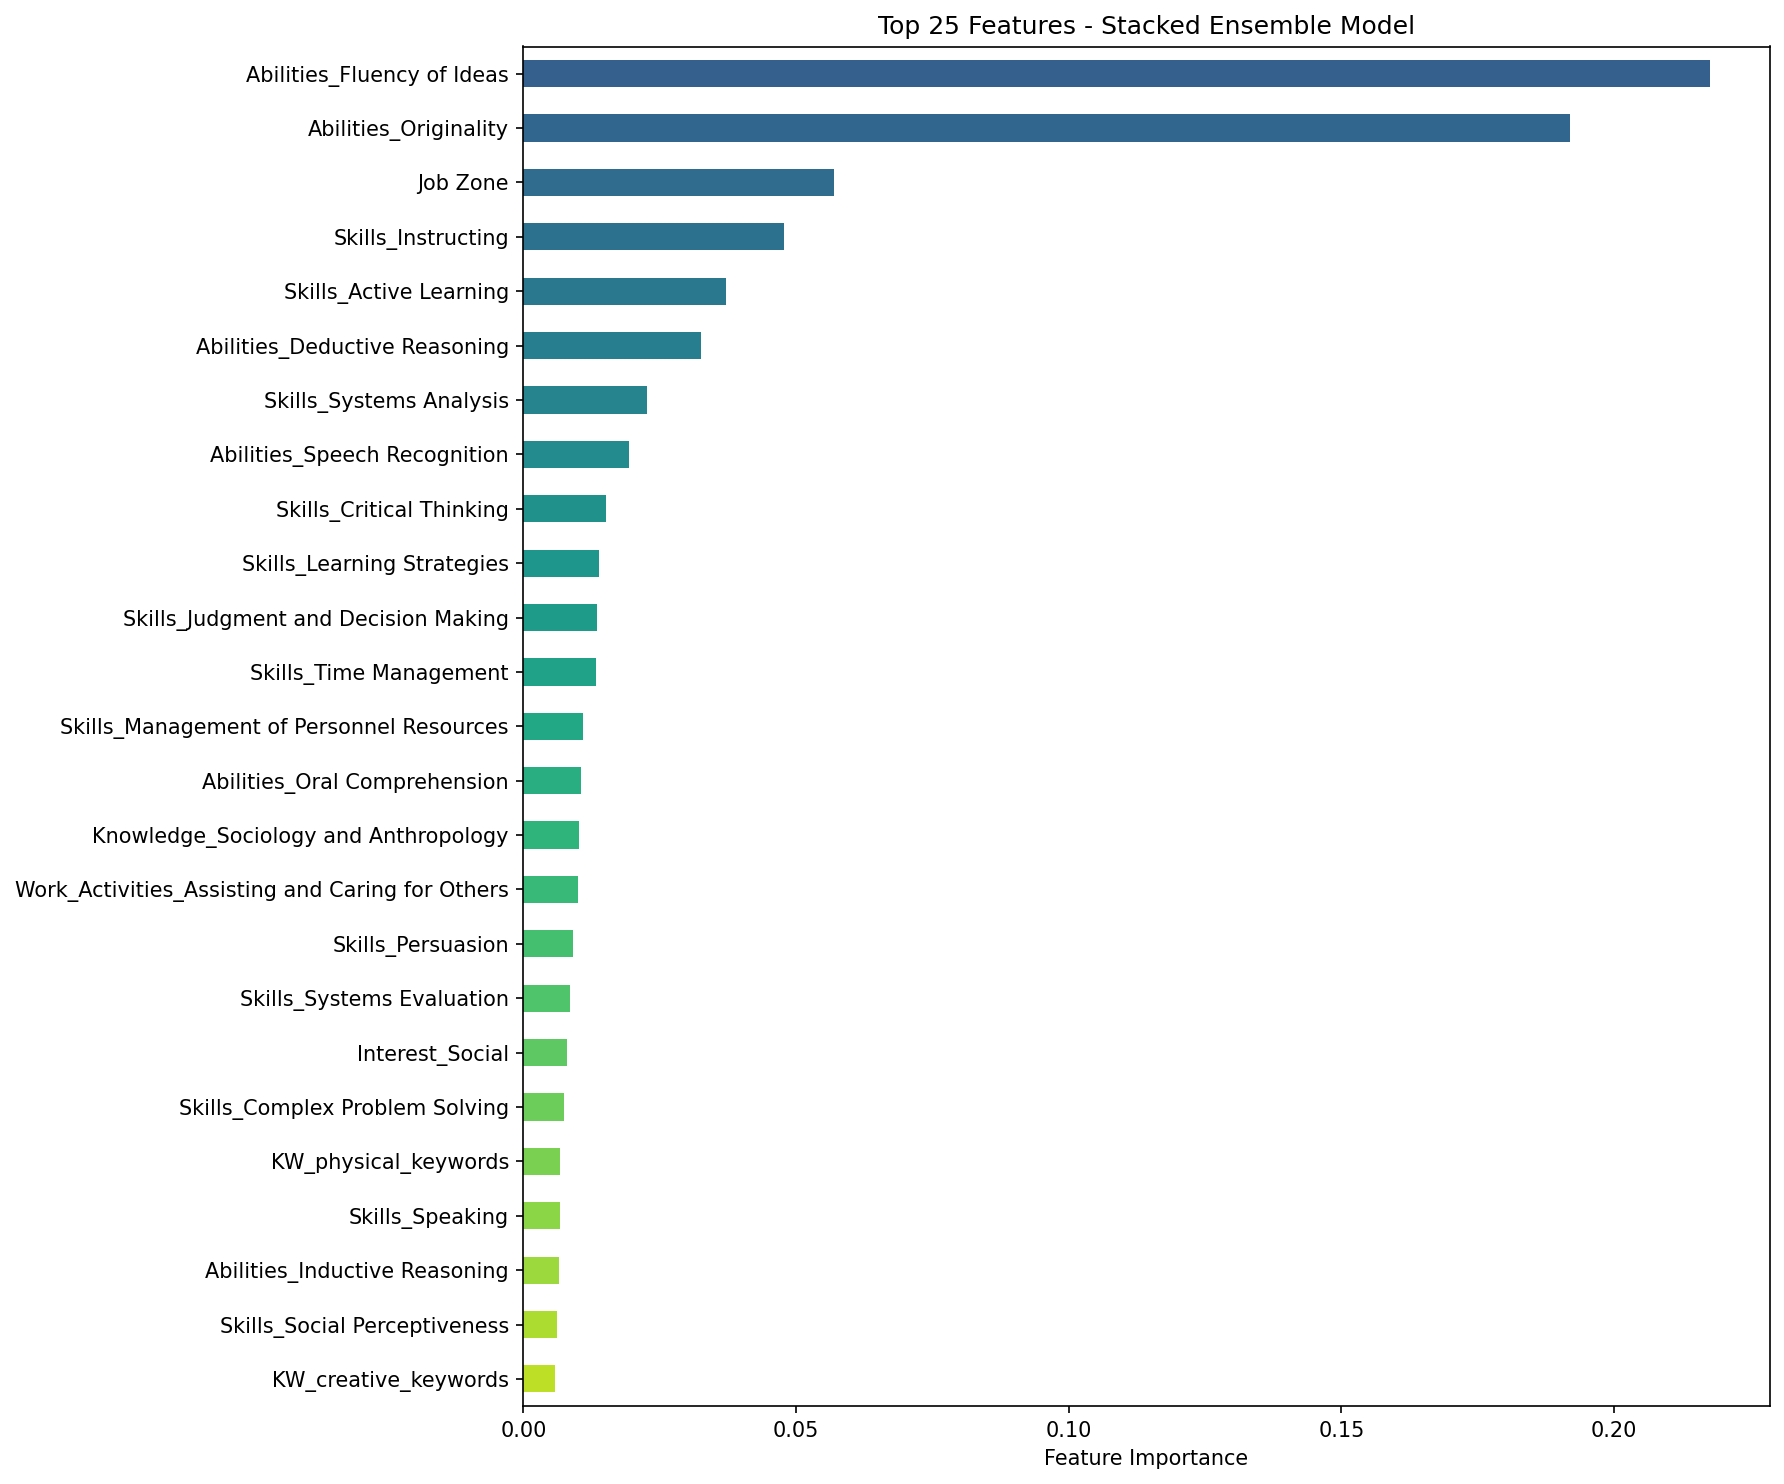
\includegraphics[width=0.85\textwidth]{images/feature_importance.png}
\caption{Feature Importance Rankings. Fluency of Ideas and Originality together account for over 40\% of the Stacked Ensemble's predictive power, confirming \citet{Frey_Osborne_2017}'s creative intelligence bottleneck.}
\label{fig:feature_importance}
\end{figure}

\section{MAEI Score Distribution}
\label{sec:maei_distribution}

Under the calibrated scenario ($W_{\text{exposure}} = 10$, $W_{\text{protection}} = 3$), the MAEI produces a mean exposure delta of $+3.86$ points across all 1,016 occupations, with 87.5\% of occupations showing a net increase in AI exposure from their 2013 baseline. This exceeds \citet{Eloundou_Manning_2023}'s estimate that 80\% of the workforce faces some LLM exposure, suggesting the MAEI's broad reach is consistent with the leading theoretical benchmark.

\begin{table}[htbp]
\centering
\caption{Sensitivity Analysis Across Uplift Weight Configurations}
\label{tab:sensitivity}
\begin{tabular}{cccc}
\toprule
$W_{\text{exposure}}$ & $W_{\text{protection}}$ & Mean Delta & \% Increased \\
\midrule
6  & 2 & $+2.26$ & 85.6\% \\
8  & 3 & $+2.77$ & 82.9\% \\
10 & 3 & $+3.86$ & 87.5\% \\
12 & 4 & $+4.38$ & 85.4\% \\
14 & 5 & $+4.89$ & 83.9\% \\
\bottomrule
\end{tabular}
\end{table}

Table~\ref{tab:sensitivity} shows that across all weight configurations tested, between 82.9\% and 87.5\% of occupations see increased exposure. The qualitative finding (that a majority of the workforce faces increased AI capability overlap) is stable regardless of the specific weight choice. The mean delta increases from $+2.26$ to $+4.89$ as weights increase, but the percentage of affected occupations remains stable, suggesting that the weights primarily affect the magnitude of exposure rather than which occupations are affected.

\begin{figure}[htbp]
\centering

\includegraphics[width=0.8\textwidth]{images/delta_distribution_corrected.png}
\caption{MAEI Score Distribution. The exposure delta distribution shows a rightward shift, with 87.5\% of occupations experiencing increased AI exposure from their 2013 baseline.}
\label{fig:delta_distribution}
\end{figure}

\begin{figure}[htbp]
\centering

\includegraphics[width=0.85\textwidth]{images/exposure_heatmap.png}
\caption{Occupation Exposure Heatmap by SOC Major Group. Office and Administrative Support (SOC 43), Business and Financial Operations (SOC 13), and Computer and Mathematical (SOC 15) occupations cluster at the highest exposure levels.}
\label{fig:heatmap}
\end{figure}

\begin{figure}[htbp]
\centering
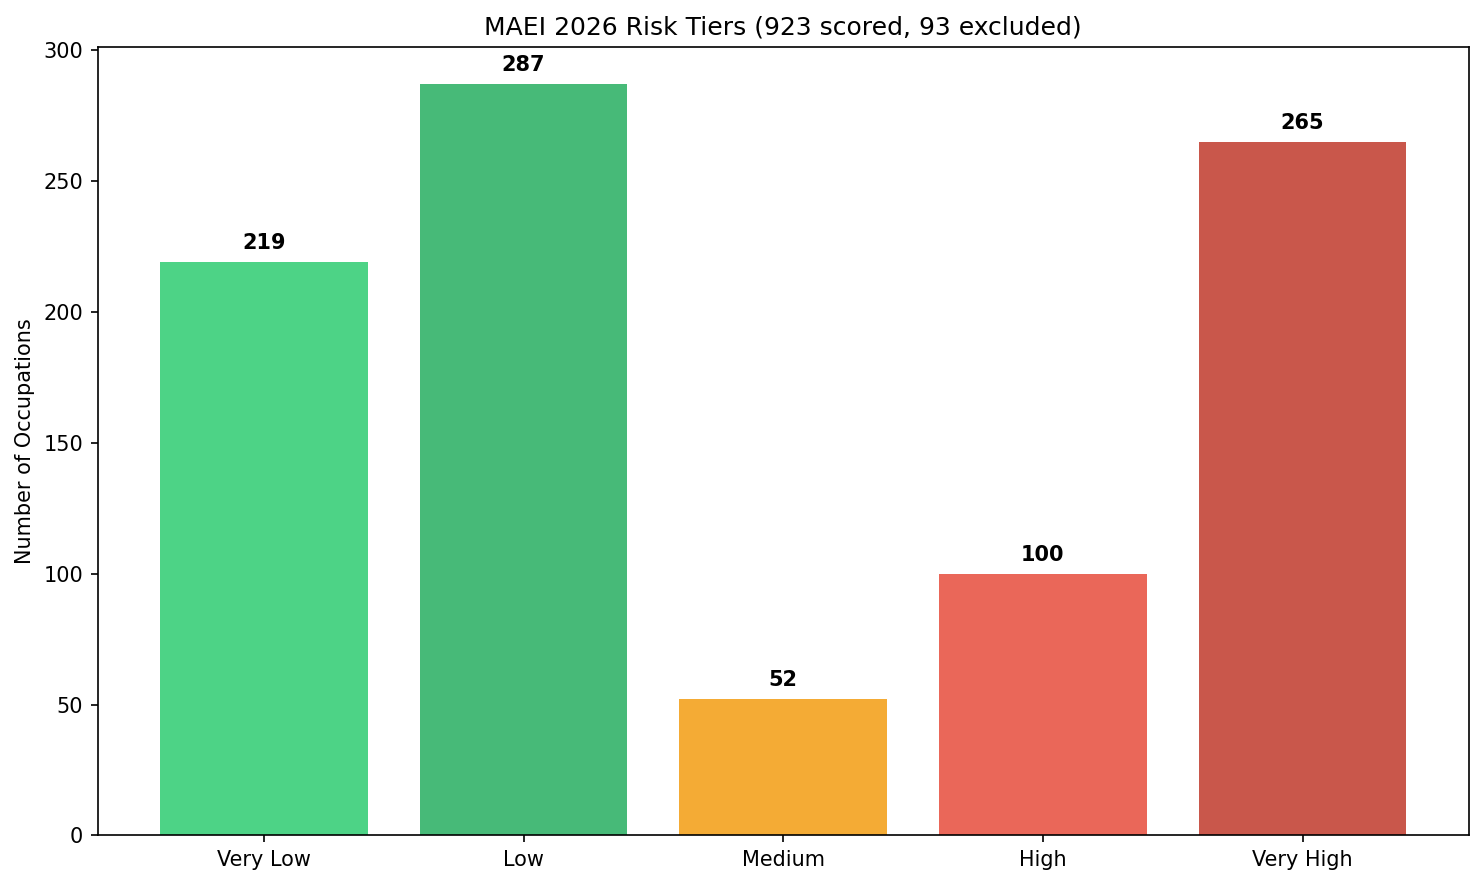
\includegraphics[width=0.7\textwidth]{images/risk_tiers_corrected.png}
\caption{Risk Tier Distribution. The bimodal pattern shows concentration at both extremes, with 265 occupations in the Very High tier and 219 in the Very Low tier.}
\label{fig:risk_tiers}
\end{figure}

The occupational extremes provide concrete illustrations of the structural inversion. Among the highest-MAEI occupations are Office Clerks (MAEI = 100.0, delta = $+4.31$), Data Entry Keyers (100.0, $+3.97$), and Claims Adjusters (100.0, $+8.07$)---all roles dominated by routine information processing that LLMs can now perform at scale. At the opposite extreme, the lowest-MAEI occupations include Makeup Artists (0.4, delta = $-0.61$), Choreographers (2.0, $+1.56$), and Preschool Teachers (1.2, $+0.43$)---roles requiring embodied physical creativity, interpersonal care, or performance artistry that remains beyond current AI capabilities. Several historically ``safe'' white-collar professions show significant exposure increases, reflecting the ceiling compression effect where the anchored scoring system caps scores at 100 while deltas continue to accumulate underneath.

\section{External Validation---The Dual-Correlation Signal}
\label{sec:external_validation}

The external validation against \citet{Felten_Raj_Seamans_2021}'s AIOE benchmark produced the strongest evidence for the MAEI's validity, testing both hypotheses simultaneously across 782 overlapping occupations.

\textbf{Anchored MAEI vs.\ AIOE: Spearman $\rho = -0.357$ ($p = 6.338 \times 10^{-25}$).} This moderate inverse correlation is the mathematical signature of the structural inversion in automation risk. The anchored MAEI retains the historical mass of the 2013 economy, where \citet{Frey_Osborne_2017} assigned the highest risk scores to manual laborers and routine workers. The AIOE, constructed from modern AI capabilities, assigns the highest exposure to cognitive and analytical workers. The negative correlation between these two measures proves that the occupational profile of risk has structurally inverted: what was safe in 2013 is exposed in 2026, and vice versa.

\textbf{Pure Exposure Delta vs.\ AIOE: Spearman $\rho = +0.764$ ($p = 1.015 \times 10^{-150}$).} When stripped of the 2013 historical anchor, the MAEI's structural model converges strongly with Felten's independently crowdsourced benchmark. Despite using entirely different methodologies (the MAEI uses scenario-based capability multipliers and an uplift formula while the AIOE uses crowdsourced human--AI task linkages), both arrive at highly correlated conclusions about which occupations face the greatest modern AI exposure. The correlation of 0.764 with a $p$-value below $10^{-150}$ is very strong.

This dual-correlation signal (negative when anchored to 2013, strongly positive when isolated to the 2026 component) is unlikely to result from noise, overfitting, or shared methodology. It provides evidence that the MAEI captures both the temporal trajectory and the contemporary reality of occupational AI exposure.

\begin{figure}[htbp]
\centering

\includegraphics[width=0.85\textwidth]{images/external_validation_aioe.png}
\caption{External Validation. The pure MAEI exposure delta shows a strong positive Spearman correlation ($\rho = +0.764$) with \citet{Felten_Raj_Seamans_2021}'s independently constructed AIOE benchmark across 782 overlapping occupations.}
\label{fig:external_validation}
\end{figure}

The strength of this dual signal becomes clearer when we consider what would happen if the MAEI were simply measuring noise. A random index would produce correlations near zero with any external benchmark, whether anchored or not. A trivially circular index that merely reproduced the same O*NET structure would show a positive correlation in both cases, not an inversion. The fact that the anchored score is negative while the pure delta is strongly positive requires a specific causal structure: the 2013 anchor must be capturing a genuinely different dimension of risk than the 2026 delta, and the 2026 delta must be capturing the same dimension as AIOE. This is precisely the inversion hypothesis: what was safe in 2013 is exposed in 2026.

\section{Structural Robustness---Multiplier Ablation}
\label{sec:multiplier_ablation}

A legitimate concern with any scenario-based model is that the results may depend critically on the specific assumptions. If the particular multiplier values I chose were driving the AIOE correlation, then changing them should alter the results. To rigorously test this, I ran seven radically different multiplier scenarios:

\begin{table}[htbp]
\centering
\caption{Multiplier Ablation Results (7 Scenarios)}
\label{tab:ablation}
\begin{tabular}{lccc}
\toprule
Scenario & Spearman $\rho$ & $p$-value & Mean Delta \\
\midrule
Baseline (Current)      & 0.7643 & $9.11 \times 10^{-151}$ & $+3.86$ \\
Halved Risk             & 0.7641 & $1.22 \times 10^{-150}$ & $+3.85$ \\
Doubled Risk            & 0.7651 & $3.02 \times 10^{-151}$ & $+3.85$ \\
Uniform Risk (all=2.0)  & 0.7637 & $2.12 \times 10^{-150}$ & $+3.81$ \\
No Protective           & 0.7636 & $2.40 \times 10^{-150}$ & $+3.78$ \\
Doubled Protective      & 0.7637 & $2.19 \times 10^{-150}$ & $+3.93$ \\
Random (seed=42)        & 0.7637 & $2.13 \times 10^{-150}$ & $+3.81$ \\
\bottomrule
\end{tabular}
\end{table}

All seven scenarios produce virtually identical correlations with AIOE, ranging from 0.7636 to 0.7651, with every $p$-value below $10^{-150}$. Whether risk multipliers are halved, doubled, set uniformly to 2.0, or replaced with random values, the relative ordering of occupations remains essentially unchanged. The occupation rankings are driven by the structural classification of features into risk and protective categories and by the binary count of features above median (the uplift formula), not by the specific numeric values of the multipliers. This converts what might initially appear as a weakness of the methodology (subjective multiplier choice) into a demonstrated strength (multiplier-invariant structural stability).

\begin{figure}[htbp]
\centering
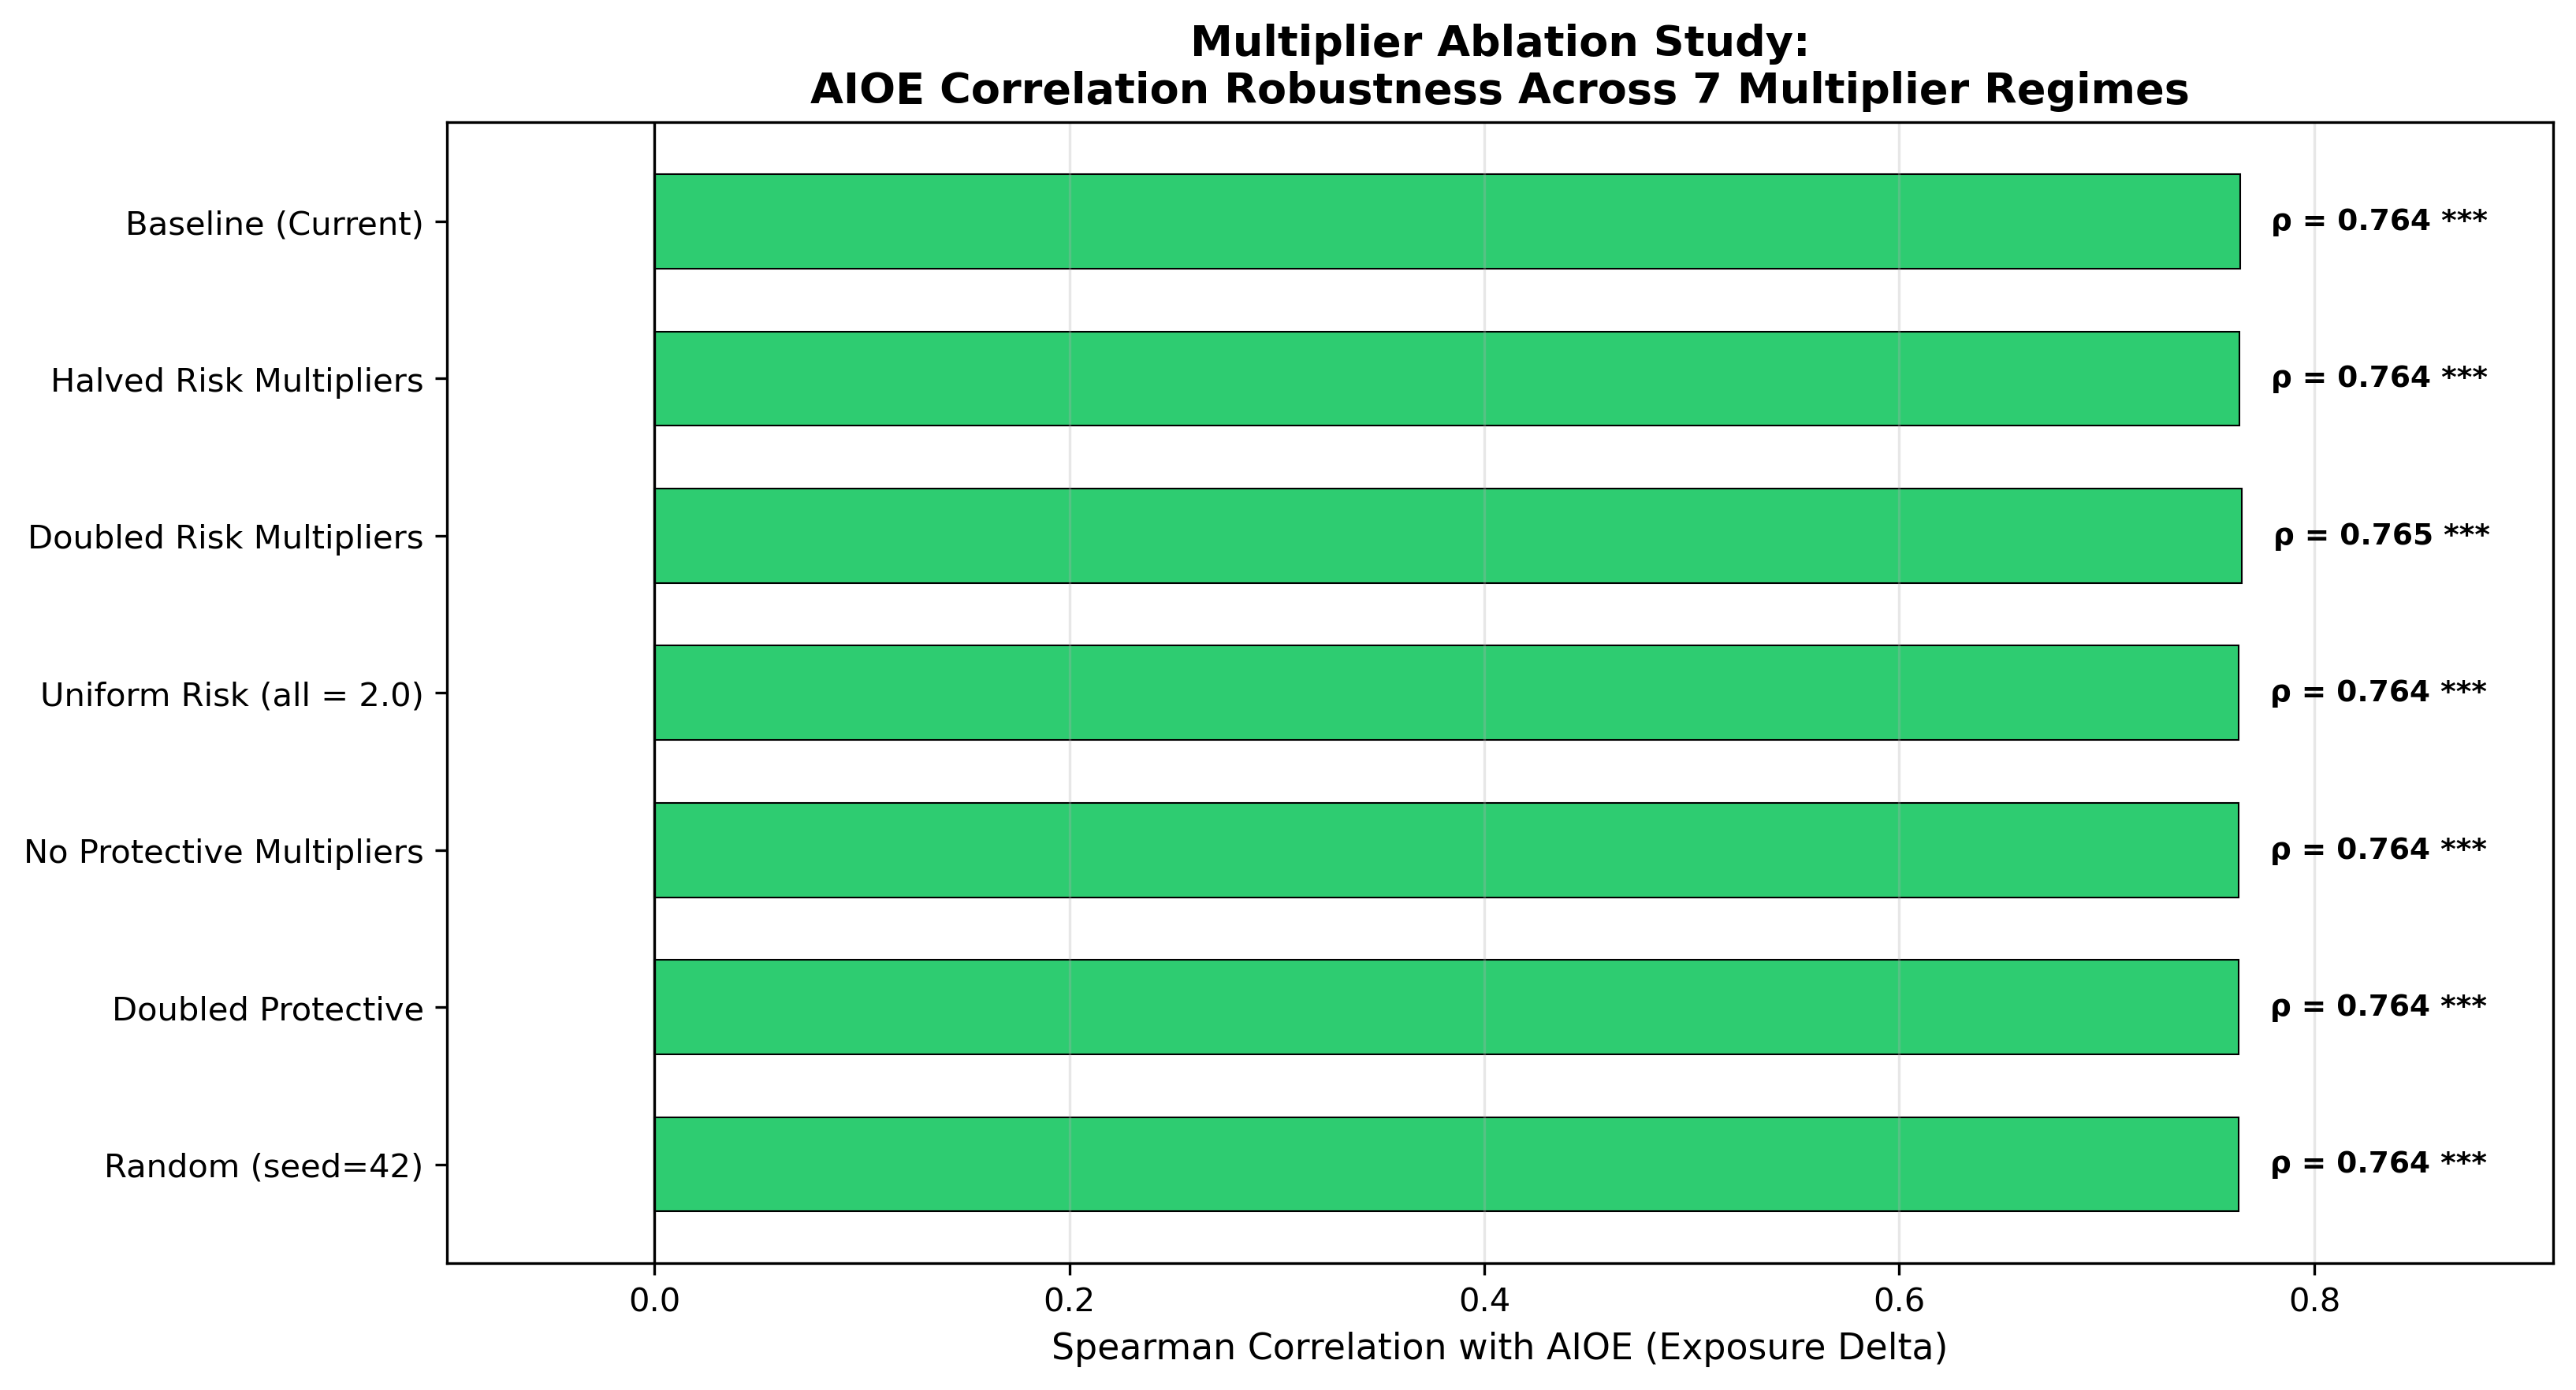
\includegraphics[width=0.8\textwidth]{images/multiplier_ablation_aioe.png}
\caption{Multiplier Ablation Study. All seven scenarios produce AIOE correlations within the narrow range of 0.7636--0.7651, demonstrating structural invariance to multiplier specification.}
\label{fig:ablation}
\end{figure}

\section{Tree Saturation---An Architectural Analysis}
\label{sec:tree_saturation}

During the stability testing phase, I discovered an important architectural property of the Stacked Ensemble that deserves careful discussion. When I compared the prediction deltas (difference between multiplied and original feature predictions) across different model architectures, the results showed a clear pattern:

\begin{table}[htbp]
\centering
\caption{Tree Extrapolation Delta Statistics by Model Architecture}
\label{tab:tree_delta}
\begin{tabular}{lccc}
\toprule
Model & Mean Delta & Std Dev & Range \\
\midrule
Ridge             & $-30.95$ & 42.33 & $[-203.2, +149.3]$ \\
XGBoost           & $+1.67$  & 4.96  & $[-15.6, +14.9]$   \\
Random Forest     & $+0.13$  & 4.73  & $[-24.8, +10.4]$   \\
Stacked Ensemble  & $+0.14$  & 0.18  & $[-0.0, +0.6]$     \\
SVR (RBF)         & $+3.41$  & 28.78 & $[-53.9, +50.1]$   \\
\bottomrule
\end{tabular}
\end{table}

The Stacked Ensemble produces deltas with a mean of just $+0.14$ and a range of essentially zero to 0.6. Compare this to Ridge Regression, which produces deltas spanning from $-203$ to $+149$. XGBoost and Random Forest are tree-based models that partition the feature space into rectangular regions during training. When a feature value is multiplied beyond the range the model saw during training (for instance, a Programming score of 100 being multiplied to 350), the tree maps it to the nearest existing leaf node, producing nearly the same prediction as before. Trees cannot extrapolate by design.

The Stacked Ensemble, whose predictions are dominated by its tree-based base learners, inherits this saturation behavior. The meta-learner (Ridge) operates on the base learners' predictions, so if the base predictions do not change, neither does the meta-learner's output. Ridge Regression alone can extrapolate linearly, producing wild deltas when features are multiplied by $3.5\times$, but there is no guarantee that such extrapolation beyond the training distribution is meaningful.

This finding explains why the three-layer architecture works. Layer 1 (the ML model) validates that Fluency of Ideas, Originality, and other key features genuinely predict 2013 automation risk. It confirms the structural plausibility of the feature set. But Layer 1 does not produce the MAEI rankings. Layer 2 (feature classification into risk versus protective categories) and Layer 3 (the uplift formula, which counts how many risk and protective features each occupation has above the median) generate the actual occupation ordering. The uplift formula operates on simple feature counts: how many risk features does this occupation have? It operates on feature counts rather than model predictions, making it immune to the tree saturation limitation.

I treat this as a methodological feature rather than a flaw. The model validates the feature selection; the uplift formula produces the rankings. Each component has a clear, defensible role, and presenting them separately is more scientifically rigorous than claiming the entire pipeline is a monolithic ``ML predicts automation'' system.

\begin{figure}[htbp]
\centering
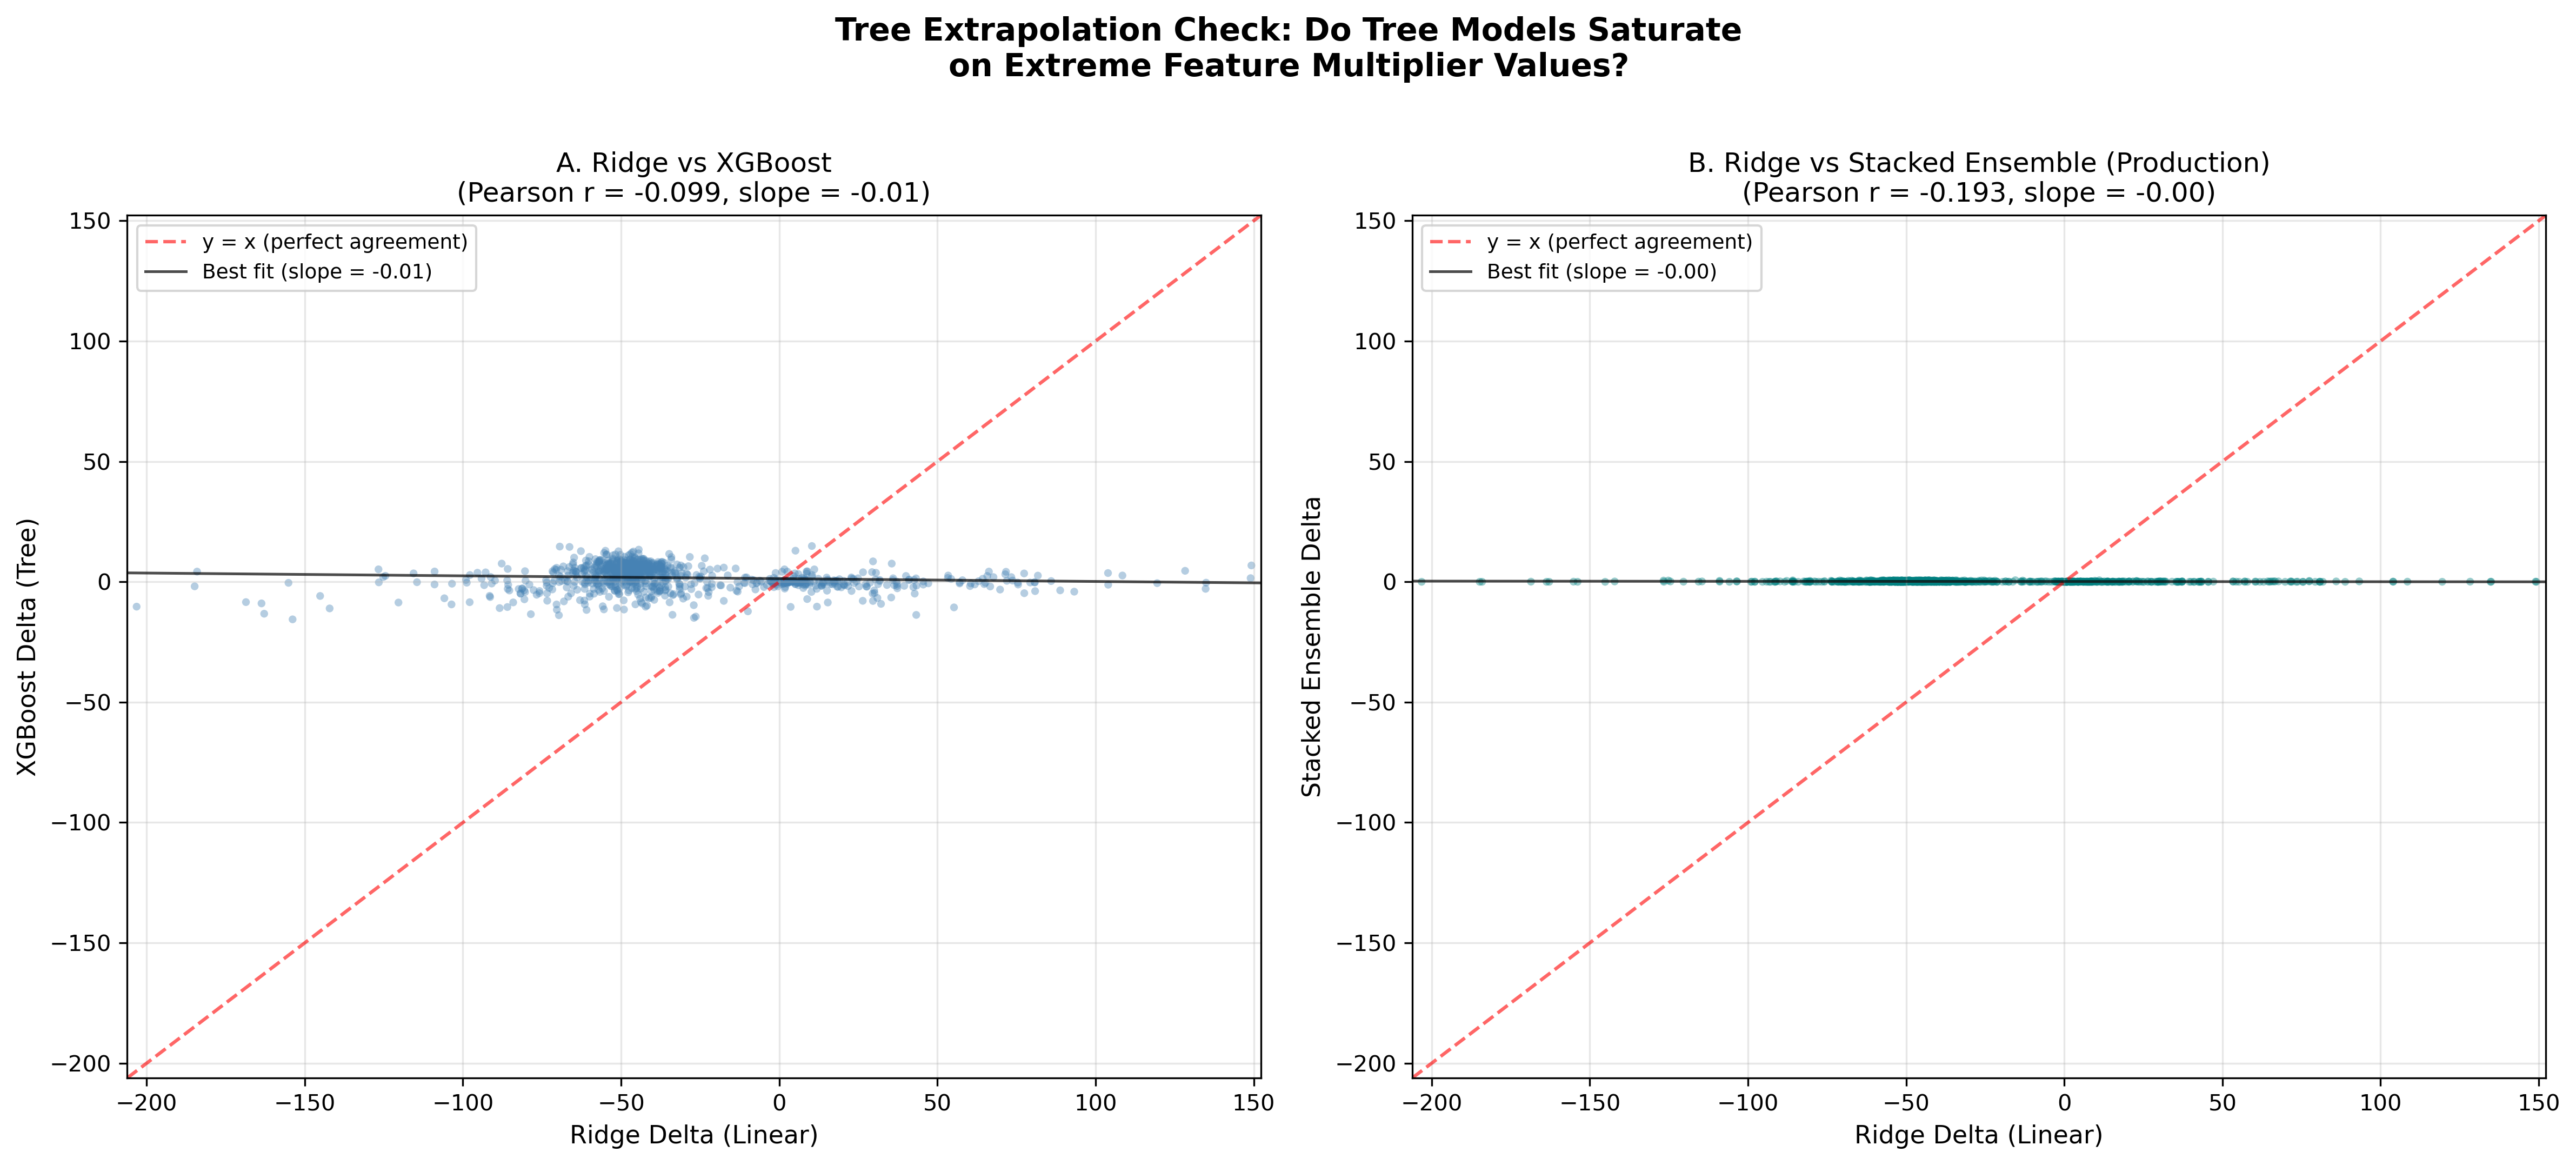
\includegraphics[width=0.85\textwidth]{images/tree_extrapolation_comparison.png}
\caption{Tree Extrapolation Comparison. Ridge Regression shows extrapolation deltas spanning $-203$ to $+149$, while the Stacked Ensemble's tree-based components produce near-zero deltas (range: $-0.0$ to $+0.6$), confirming the saturation hypothesis.}
\label{fig:tree_extrapolation}
\end{figure}

\section{Discussion}
\label{sec:discussion}

Collectively, these results support three conclusions. First, the occupational profile of AI exposure has structurally inverted since 2013. The jobs \citet{Frey_Osborne_2017} identified as safe (cognitive, analytical, communicative) are precisely the ones the MAEI identifies as most exposed under 2026 conditions. This finding aligns with \citet{Felten_Raj_Seamans_2021}, \citet{Eloundou_Manning_2023}, and \citeauthor{Anthropic_2026}'s \citeyearpar{Anthropic_2026} independent analyses using different data and methods.

Second, the MAEI's occupation rankings are structurally stable. The seven-scenario ablation study proves that the rankings are invariant to multiplier specification; regardless of whether multiplier values are halved, doubled, randomized, or set uniformly, the same occupations end up at the top and bottom of the exposure distribution. This stability stems from the feature classification layer (risk vs.\ protective) and the uplift formula, which depend on which features are classified as risk or protective and how many of them each occupation possesses, not on the specific multiplier magnitudes.

Third, the three-layer architecture demonstrates a methodologically explicit approach to scenario-based indexing. By explicitly documenting the tree saturation phenomenon and separating the model's validation role from the uplift formula's ranking role, the MAEI avoids the common pitfall of over-claiming what the machine learning component actually contributes. This decomposition makes the index more interpretable and more defensible than a black-box approach would be.
